The phases of matter are characterised by two symmetry groups - $G$, the symmetry of the free energy of the system and $H$, the symmetry of the ground state.\\

\noindent This structure can be seen in the Ising model. When $B=0$, the free energy has a $G=\mathbb{Z}_2$ symmetry. In the disordered phase this symmetry is unbroken, i.e. $H=\mathbb{Z}_2$ also. In contrast, in the ordered phase the symmetry is spontaneously broken as the system must choose one of two ground states. Here $H$ has no symmetry group.\\ 

\noindent Whenever a discrete symmetry group is spontaneously broken, it results in multiple ground states. One can move from one ground state to another by acting with the broken generators of $G$. The different phases of matter within this class are characterised by $H$, therefore there must be a phase transition, whenever $H$ changes.\\

\noindent The theory of $N$ real scalar fields with $O(N)$ symmetry can be used to demonstrate spontaneuos symmetry breaking in condensed matter systems. The $N=2$ models come under the $XY$-universality class. Bose-Einstein condensates and superfluids are described in this way.\\ 

\noindent It is convenient to pair the two real fields as one complex field as $\psi=\phi_1+i\phi_2$. This is now invariant under $U(1)$ transformations, $\psi'=e^{i\theta}\psi$. Unlike the Ising model, where there were only two possible ground states, in a continuous symmetry there are an infinite number of ground states.\\ 

\noindent The minimum of the free energy constrains only the magnitude of $\psi$ which is given by $\langle|\psi|\rangle=M_0=\sqrt{\frac{-\mu^2}{4g}}$. However, minimising the free energy does not determine the direction of $\psi$. We are left with a space of ground states which is the sphere $\mathbb{S}^{N-1}=\frac{O(N)}{O(N-1)}$. In a general sense, the manifold of ground states is given by $\frac{G}{H}$. Each point on the sphere, parameterizes the direction of $\psi$ and has the same energy.\\

\noindent We can consider configurations in which we stay within the space of ground states, but the direction varies in space. For such configurations, the part of the free energy $f(\psi)=\mu^2|\psi|^2+g|\psi|^4$ remains minimised, but we pick up contributions from the gradient terms $\nabla\psi^*\nabla\psi$.\\

\noindent These kind of excitations, which arise from the spontaneous breaking of continuous symmetries, are known as Goldstone bosons. The number of Goldstone bosons is given as $\text{dim}(G)-\text{dim}(H)$. For the $O(N)$ models, the number is $\frac{1}{2}N(N-1)-\frac{1}{2}(N-1)(N-2)=N-1$, which is the dimensionality of $\mathbb{S}^{N-1}$.\\

\begin{center}
    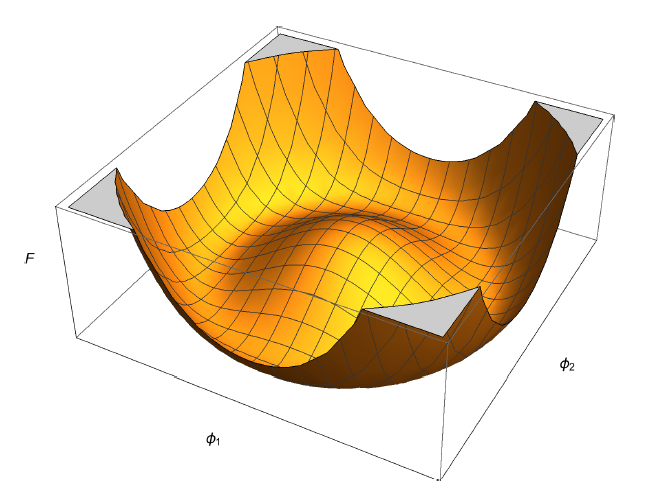
\includegraphics[scale=0.8]{ssb}
\end{center}

\noindent For the $XY$ class, in the ordered phase we get a free energy of the form as shown above. There is a circle of minima, $\mathbb{S}^1$. If we write $\psi(\boldsymbol{x})=M(\boldsymbol{x})e^{i\theta(\boldsymbol{x})}$ and $M(\boldsymbol{x})=M_0+\bar{M}(\boldsymbol{x})$, the free energy takes the form,

$$F[M,\theta]=\int d^dx\,\frac{\gamma}{2}(\nabla\bar{M})^2+\mu^2\bar{M}^2+g\bar{M}^4+\frac{\gamma}{2}M_0^2(\nabla\theta)^2+\gamma M_0\bar{M}(\nabla\theta)^2$$

\noindent $\theta$ is the Goldstone boson.